\chapter{RESPOSTAS DA PESQUISA DE INFORMAÇÕES}
\label{ap:respostas}

Este apêndice apresenta os resultados coletados através do formulário de pesquisa sobre hábitos de uso de dispositivos móveis aplicado a um grupo de participantes representativos do público-alvo do aplicativo Desconecta.

\vspace{1cm}

\begin{center}
    \textbf{Respostas da Pergunta 1}
\end{center}

\vspace{0.3cm}

\noindent Você sente que passa mais tempo no celular do que gostaria?

\begin{figure}[H]
    \centering
    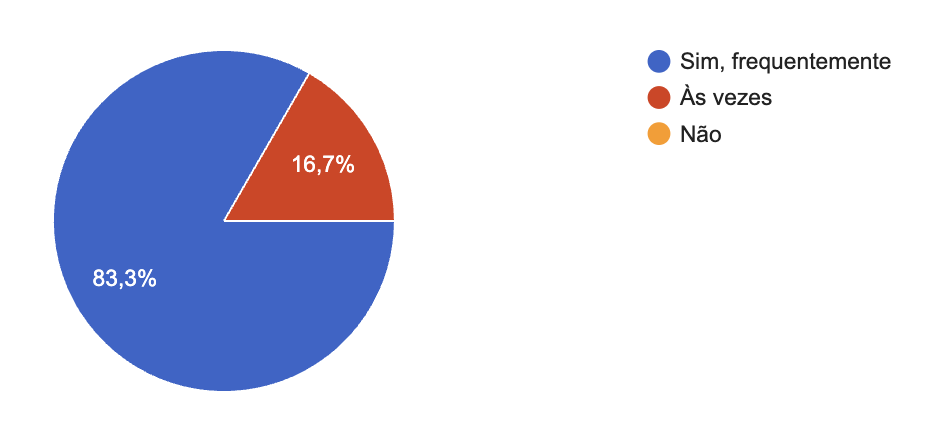
\includegraphics[width=0.7\textwidth]{figuras/uso_excessivo.png}
\end{figure}

\vspace{0.8cm}

\begin{center}
    \textbf{Respostas da Pergunta 2}
\end{center}

\vspace{0.3cm}

\noindent Com que frequência você pega o celular sem um motivo específico (por tédio, hábito, costume)?

\begin{figure}[H]
    \centering
    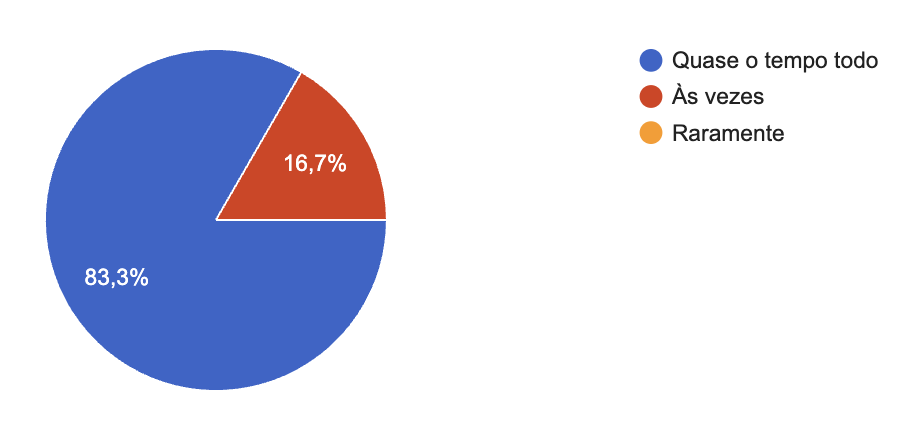
\includegraphics[width=0.7\textwidth]{figuras/uso_sem_motivo.png}
\end{figure}

\vspace{0.8cm}

\begin{center}
    \textbf{Respostas da Pergunta 3}
\end{center}

\vspace{0.3cm}

\noindent Você já sentiu ansiedade ou desconforto ao ficar longe do celular?

\begin{figure}[H]
    \centering
    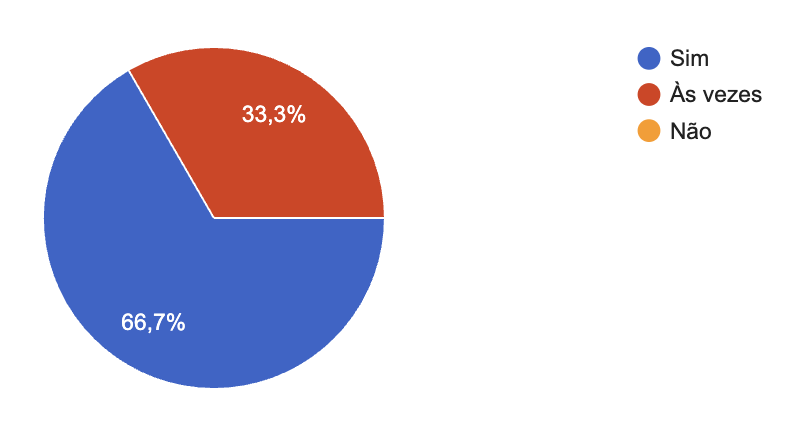
\includegraphics[width=0.7\textwidth]{figuras/ansiedade_longe_celular.png}
\end{figure}

\vspace{0.8cm}

\begin{center}
    \textbf{Respostas da Pergunta 4}
\end{center}

\vspace{0.3cm}

\noindent Qual dessas situações acontece com você com mais frequência? (pode marcar mais de uma)

\begin{figure}[H]
    \centering
    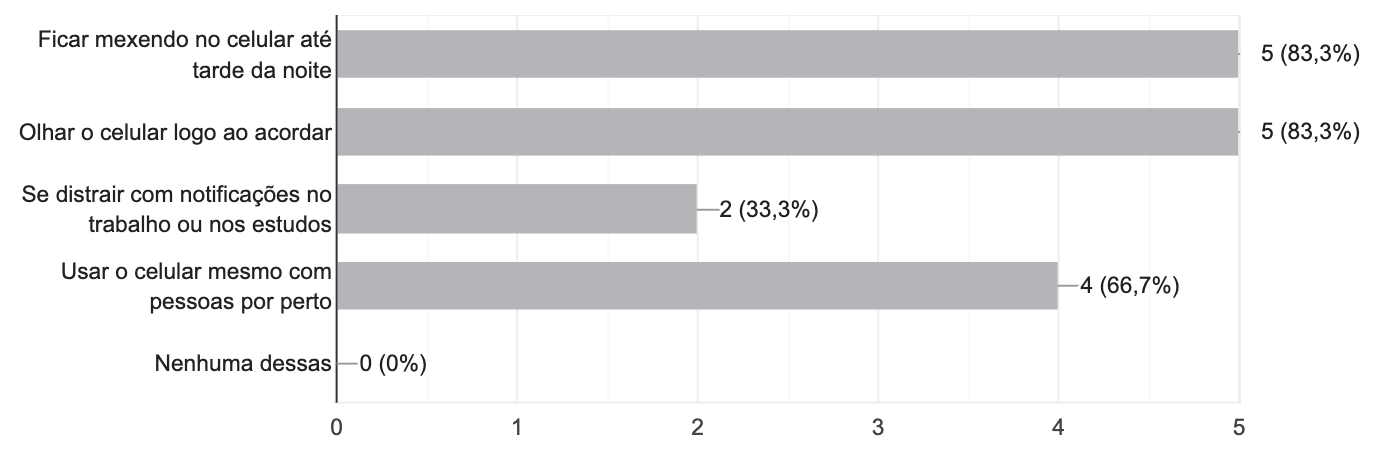
\includegraphics[width=0.7\textwidth]{figuras/situacoes_mais_frequentes.png}
\end{figure}

\vspace{0.8cm}

\begin{center}
    \textbf{Respostas da Pergunta 5}
\end{center}

\vspace{0.3cm}

\noindent Você já tentou reduzir o tempo de uso do celular por conta própria?

\begin{figure}[H]
    \centering
    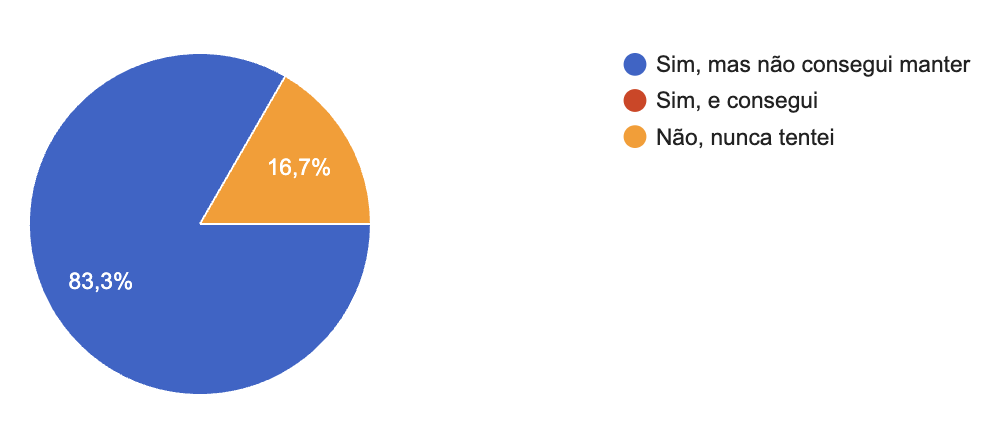
\includegraphics[width=0.7\textwidth]{figuras/ja_tentou_reduzir_sozinho.png}
\end{figure}

\vspace{0.8cm}

\begin{center}
    \textbf{Respostas da Pergunta 6}
\end{center}

\vspace{0.3cm}

\noindent O que mais te motivaria a usar menos o celular?

\begin{figure}[H]
    \centering
    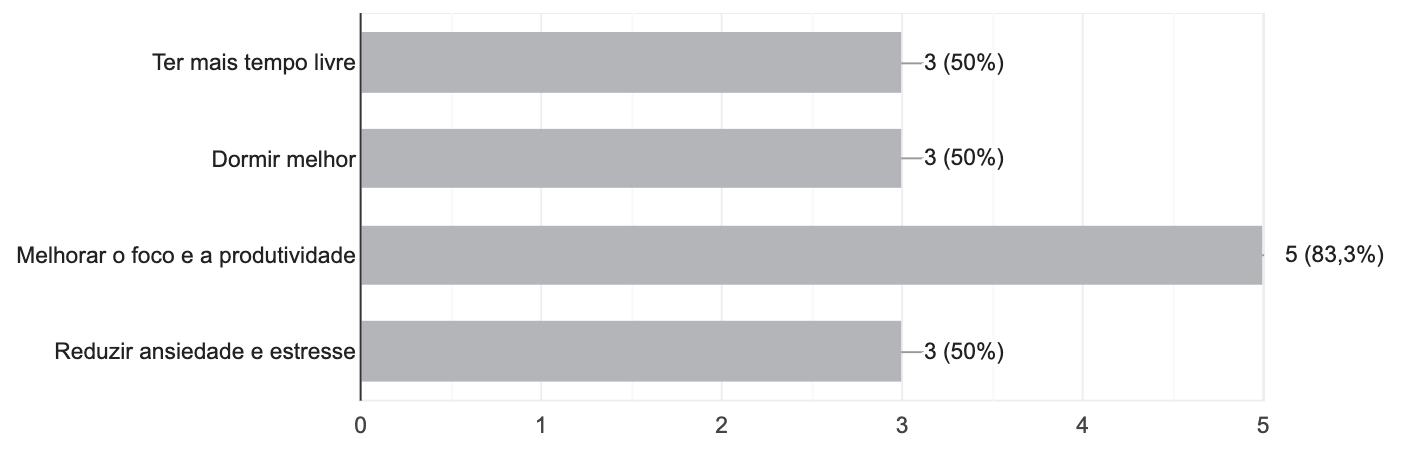
\includegraphics[width=0.7\textwidth]{figuras/oq_mais_motiva_usar_menos.png}
\end{figure}

\vspace{0.8cm}

\begin{center}
    \textbf{Respostas da Pergunta 7}
\end{center}

\vspace{0.3cm}

\noindent Você acha que participar de um desafio em grupo focado na redução do tempo de tela pode ajudar você a usar menos o celular?

\begin{figure}[H]
    \centering
    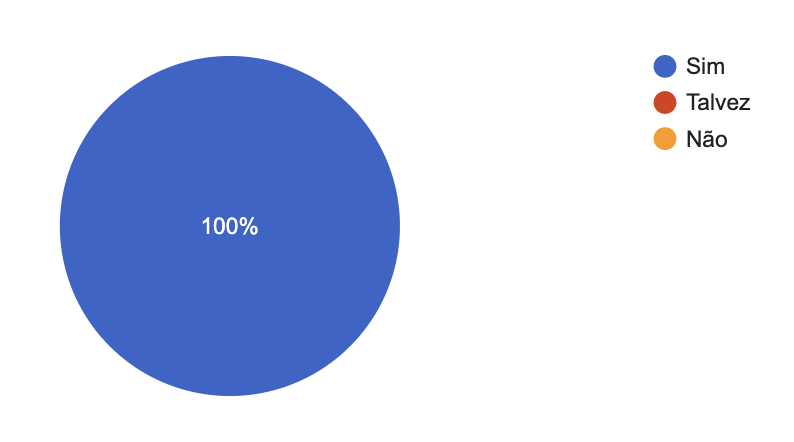
\includegraphics[width=0.7\textwidth]{figuras/grupo_ajuda.png}
\end{figure}

\vspace{0.8cm}

\begin{center}
    \textbf{Respostas da Pergunta 8}
\end{center}

\vspace{0.3cm}

\noindent Ver outras pessoas compartilhando o próprio tempo de tela te motivaria a reduzir o seu também?

\begin{figure}[H]
    \centering
    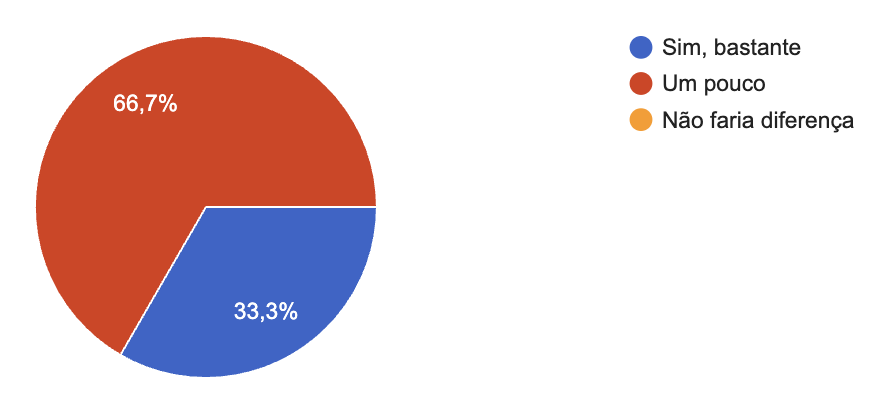
\includegraphics[width=0.7\textwidth]{figuras/motivacao_comparacao.png}
\end{figure}

\vspace{0.8cm}

\begin{center}
    \textbf{Respostas da Pergunta 9}
\end{center}

\vspace{0.3cm}

\noindent Você se sente mais motivado(a) quando está em um grupo com o mesmo objetivo?

\begin{figure}[H]
    \centering
    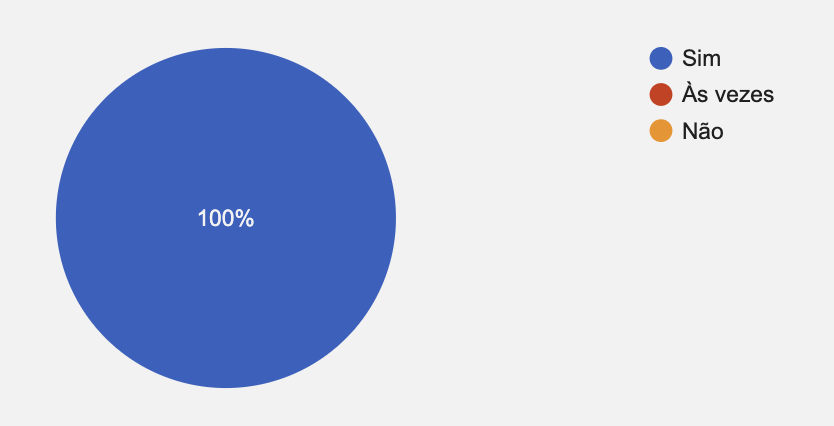
\includegraphics[width=0.7\textwidth]{figuras/motivacao_grupo.png}
\end{figure}

\vspace{0.8cm}

\begin{center}
    \textbf{Respostas da Pergunta 10}
\end{center}

\vspace{0.3cm}

\noindent Saber que outras pessoas podem ver o seu tempo de tela faria você usar menos o celular?

\begin{figure}[H]
    \centering
    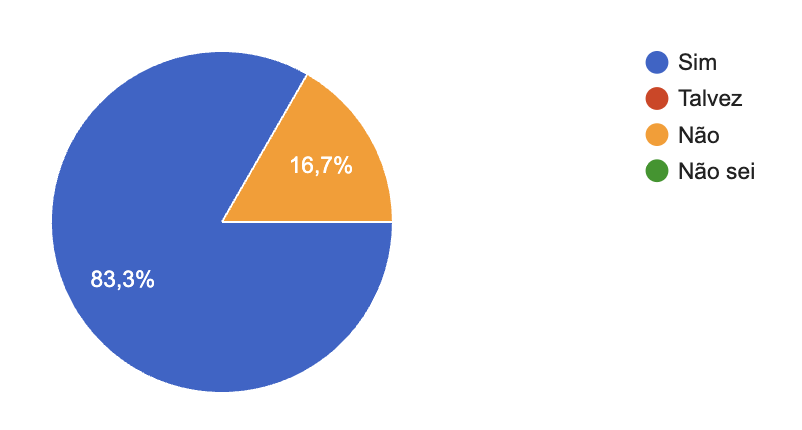
\includegraphics[width=0.7\textwidth]{figuras/visibilidade_social.png}
\end{figure}

\vspace{0.8cm}

\begin{center}
    \textbf{Respostas da Pergunta 11}
\end{center}

\vspace{0.3cm}

\noindent Você concorda com a ideia de participar de um grupo onde as pessoas se apoiam e compartilham a redução diária do tempo de tela?

\begin{figure}[H]
    \centering
    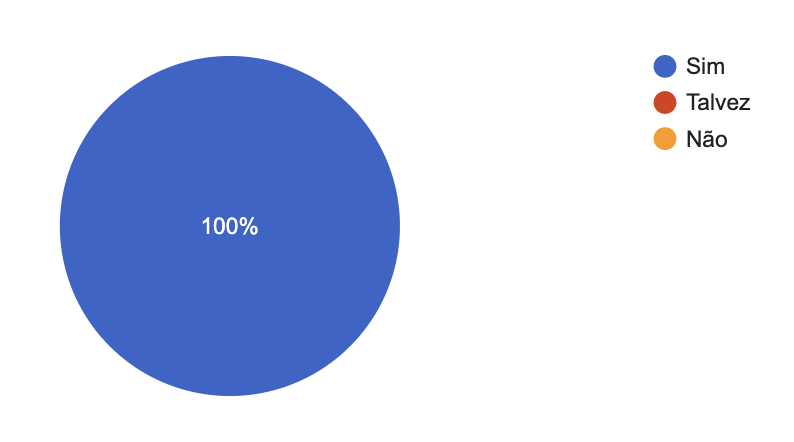
\includegraphics[width=0.7\textwidth]{figuras/grupo_ajuda.png}
\end{figure}

\vspace{0.8cm}

\begin{center}
    \textbf{Respostas da Pergunta 12}
\end{center}

\vspace{0.3cm}

\noindent O que mais te ajudaria em um grupo focado em usar menos o celular?

\begin{figure}[H]
    \centering
    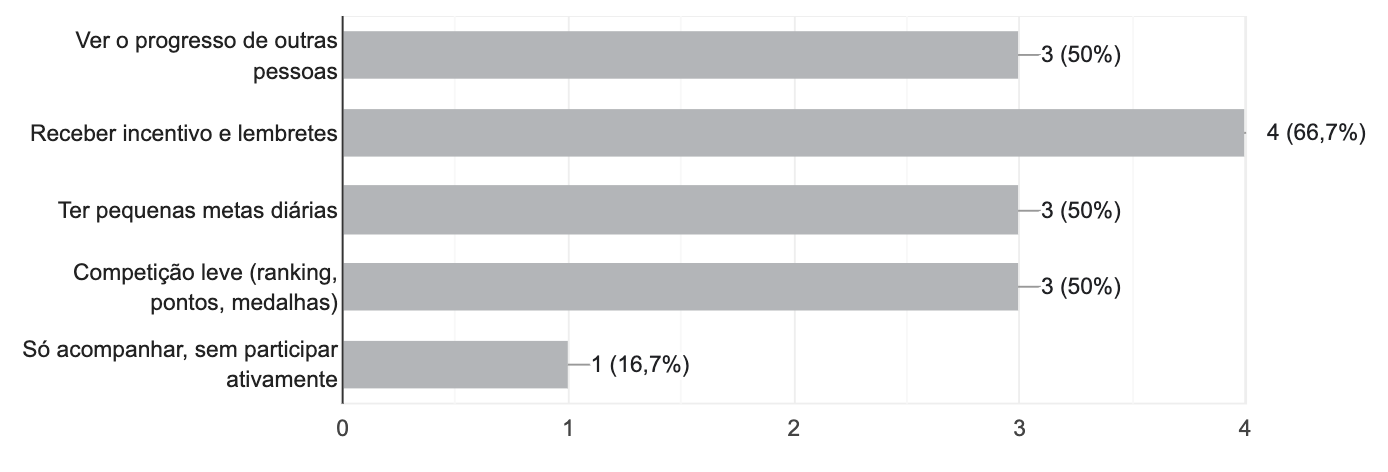
\includegraphics[width=0.7\textwidth]{figuras/elementos_grupo.png} %mesmo resultado da pergunta 7
\end{figure}